\documentclass{standalone}
\usepackage{tikz}
\usetikzlibrary{shapes.geometric,decorations.markings,arrows,positioning}

\tikzset{
    buffer/.style={
        draw,
        regular polygon,
        regular polygon sides=3,
        node distance=3cm,
        minimum height=6em
    }
}

\begin{document}
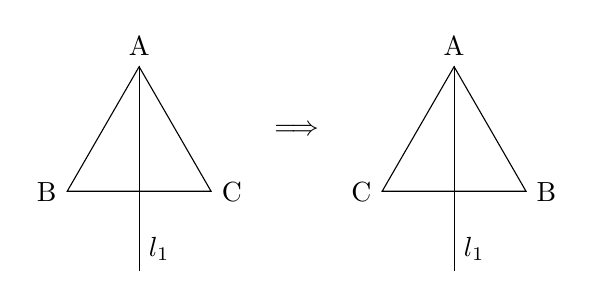
\begin{tikzpicture}
  \node[buffer] (T) {};
  \node at (T.corner 1)(A)[above]{A};
  \node at (T.corner 2)(B)[left]{B};
  \node at (T.corner 3)(C)[right]{C};
  \draw (A) -- (B-|A) -- ++(-90:1cm) node[above right] {$l_1$};

  \node at (2,0.25) (Arr) {$\Longrightarrow$};

  \begin{scope}[xshift=4cm];
    \node[buffer] (T1) {};
    \node at (T1.corner 1) (A1) [above] {A};
    \node at (T1.corner 2) (B1) [left] {C};
    \node at (T1.corner 3) (C1) [right] {B};
    \draw (A1) -- (B1-|A1) -- ++(-90:1cm) node[above right] {$l_1$};
  \end{scope}

\end{tikzpicture}
\end{document}
